\documentclass[11pt,a4paper]{article}

% --- Core Packages ---
\usepackage[utf8]{inputenc}
\usepackage[margin=1in]{geometry}
\usepackage{amsmath,amssymb,amsfonts}
\usepackage{graphicx}
\usepackage{booktabs}
\usepackage{hyperref}
\usepackage{subcaption}
\usepackage{cite}
\usepackage{xcolor}
\usepackage{float}
\usepackage{listings}
\usepackage{microtype}

\hypersetup{
    colorlinks=true,
    linkcolor=blue,
    citecolor=blue,
    urlcolor=blue,
    pdftitle={Consolidated Project Report: Multi-Objective Bayesian Optimization for a 200 MeV Electron Injector Linac},
    pdfauthor={Chong Shik Park}
}

% --- Code Listing Setup ---
\lstset{
    basicstyle=\ttfamily\small,
    breaklines=true,
    frame=single,
    backgroundcolor=\color{gray!10},
    keywordstyle=\color{blue},
    commentstyle=\color{green!60!black},
    stringstyle=\color{purple}
}

\title{\textbf{Consolidated Project Report \& Simulation Architecture:\\ Multi-Objective Bayesian Optimization for a 200~MeV Electron Injector Linac}}

\author{\textbf{Chong Shik Park}\\
    Department of Accelerator Science, Korea University, Sejong 30019, South Korea\\
    \texttt{kuphy@korea.ac.kr}
}

\date{\today}

\begin{document}

\maketitle

\begin{abstract}
This consolidated document provides a comprehensive technical overview of the Machine Learning framework developed for optimizing a 200~MeV S-band electron injector linac using Multi-Objective Bayesian Optimization (MOBO). Synthesizing physics modeling, literature background, software architecture, simulation execution protocols, and verification methods, this report details the progression from initial scalarized Bayesian Optimization presented at ICABU 2025 to parallel $q\text{LogNEHVI}$-based MOBO with explicit Gaussian Process constraint modeling. Key architectural innovations include isolated per-evaluation working directory management to prevent parallel simulation file races, canonical physical-to-model space objective transformations, fixed reporting reference point standards, and independent Pareto candidate verification. All 5 selected representative Pareto front candidates achieve exact numerical reproducibility ($<10^{-6}\%$ relative error), establishing a reliable foundation for automated accelerator design and future high-performance computing deployment.
\end{abstract}

\tableofcontents
\newpage

% ==============================================================================
\section{Introduction \& Project Overview}
\label{sec:introduction}
% ==============================================================================

High-brightness electron injector linear accelerators (linacs) serve as the critical driver for modern light sources, including X-ray Free-Electron Lasers (XFELs), ultrafast electron diffraction (UED) systems, and industrial beamlines. Producing high-quality electron beams requires simultaneous optimization of conflicting beam quality metrics: minimizing horizontal normalized emittance ($\varepsilon_{n,x}$), vertical normalized emittance ($\varepsilon_{n,y}$), and RMS energy spread ($\sigma_E$), while satisfying strict constraints on beam envelope sizes, bunch length, mean kinetic energy, and transmission efficiency.

Traditionally, linear accelerator parameters have been tuned manually or optimized using heuristic scalarization methods (e.g., weighted-sum single-objective Bayesian Optimization or Multi-Objective Genetic Algorithms like MOGA). However, pre-defined objective weighting biases candidate selection and conceals the global Pareto front topology. True Multi-Objective Bayesian Optimization (MOBO) leverages independent Gaussian Process (GP) surrogates to efficiently explore non-dominated trade-offs while drastically reducing expensive particle tracking simulation budgets.

Preliminary scalarized BO research was presented at **ICABU 2025** \cite{ICABU2025}. This framework has since evolved into a production-grade Python package (\texttt{mobo\_linac}) featuring:
\begin{enumerate}
    \item \textbf{Process-Safe Directory Isolation}: Dedicated evaluation subdirectories (\texttt{results/<run\_id>/work/eval\_<id>/}) preventing file race conditions during multi-core parallel execution.
    \item \textbf{Strict Failure Semantics}: Explicit separation of numerical simulation convergence from physical beam feasibility.
    \item \textbf{Fixed Hypervolume Tracking}: Fixed reporting reference point standard ($\mathbf{r}_{\text{rep}} = [1.5\text{ mm}, 1.5\text{ mm}, 1.5\text{ MeV}]$) ensuring un-biased hypervolume growth monitoring.
    \item \textbf{Independent Pareto Verification}: Automated re-simulation protocol verifying candidate reproducibility down to $10^{-6}\%$ relative difference.
\end{enumerate}

% ==============================================================================
\section{Physics Models \& Accelerator Specification}
\label{sec:physics}
% ==============================================================================

\subsection{Linac Mechanical \& Optical Layout}
The 200~MeV S-band electron injector linac model consists of:
\begin{itemize}
    \item **RF Photo-Gun**: 1.5-cell S-band ($2.856$~GHz) photo-cathode RF cavity generating high-brightness electron bunches.
    \item **Solenoid Magnet**: Peak field $B_{\text{sol}}$ located at the gun exit for emittance compensation.
    \item **Accelerating Cavities (ACC1--ACC4)**: Four traveling-wave structures (TWS) boosting kinetic energy to 200~MeV. Cavities 1--2 and Cavities 3--4 share coupled RF phase controls ($\phi_{\text{acc1/2}}$ and $\phi_{\text{acc3/4}}$).
    \item **Quadrupole Doublet**: Focusing magnetic gradients ($G_{q1}, G_{q2}$) downstream for beam envelope control.
\end{itemize}

\subsection{Design Parameters (6D Control Space)}
The 6 continuous optimization variables written into the ASTRA input template (\texttt{astra.in}) before each simulation run are detailed in Table~\ref{tab:design_variables}.

\begin{table}[H]
\centering
\caption{Design parameter definitions, ASTRA key mappings, nominal values, and search bounds.}
\label{tab:design_variables}
\begin{tabular}{lccccc}
\toprule
\textbf{Variable Description} & \textbf{ASTRA Input Variable} & \textbf{Nominal} & \textbf{Lower} & \textbf{Upper} & \textbf{Unit} \\
\midrule
Solenoid Peak Field & \texttt{solenoid:maxb(1)} & 0.1948 & 0.0974 & 0.2922 & T \\
Quadrupole 1 Gradient & \texttt{quadrupole:q\_grad(1)} & 1.2865 & 0.6433 & 1.9298 & T/m \\
Quadrupole 2 Gradient & \texttt{quadrupole:q\_grad(2)} & -2.8867 & -4.3300 & -1.4433 & T/m \\
RF Gun Phase & \texttt{cavity:phi(1)} & 35.62 & 32.06 & 39.19 & deg \\
ACC1/ACC2 Coupled Phase & \texttt{cavity:phi(2,3)} & -39.51 & -43.46 & -35.56 & deg \\
ACC3/ACC4 Coupled Phase & \texttt{cavity:phi(4,5)} & 310.05 & 279.05 & 341.06 & deg \\
\bottomrule
\end{tabular}
\end{table}

\subsection{Particle Tracking \& Space Charge Settings}
Simulations are performed using ASTRA (v3.2) \cite{AstraManual} wrapped via \texttt{lume-astra}. Initial particle distributions (\texttt{pal\_photo2.ini}) represent $N = 10,000$ macroparticles with a total bunch charge $Q = 250$~pC. Space-charge forces are computed using a 2D cylindrical mesh solver ($N_r = 25, N_z = 50$). Field distributions for gun, solenoid, and accelerating structures are provided by realistic field map files (\texttt{gun.dat}, \texttt{PAL\_SOL\_A.dat}, \texttt{TWS\_Sband.dat}). Final diagnostics are evaluated at $s = 16.20$~m.

% ==============================================================================
\section{Objective Conventions \& Constraint Rationales}
\label{sec:objectives_constraints}
% ==============================================================================

\subsection{Physical vs. Model Space Canonical Transformations}
The physical optimization problem minimizes three beam quality objectives:
\begin{equation}
    \mathbf{y}_{\text{phys}}(\mathbf{x}) = \left[ \varepsilon_{n,x}(\mathbf{x}),\, \varepsilon_{n,y}(\mathbf{x}),\, \sigma_E(\mathbf{x}) \right]^\top
\end{equation}

Because BoTorch \cite{Botorch2020} assumes objective maximization, all physical objectives are transformed to model space via canonical negation:
\begin{equation}
    \mathbf{y}_{\text{model}} = -\mathbf{y}_{\text{phys}} = \left[ -\varepsilon_{n,x},\, -\varepsilon_{n,y},\, -\sigma_E \right]^\top
\end{equation}
Physical objective values remain strictly positive ($\varepsilon_{n,x}, \varepsilon_{n,y} > 0, \sigma_E > 0$).

\subsection{Beam Quality Constraint Formulation}
A simulation outcome must satisfy 8 physical constraints to be classified as physically feasible:
\begin{align}
    \sigma_x &\le 1.0\text{ mm}, & \sigma_y &\le 1.0\text{ mm}, \\
    \sigma_{x'} &\le 1.0\text{ mrad}, & \sigma_{y'} &\le 1.0\text{ mrad}, \\
    \sigma_z &\le 1.0\text{ mm}, & 195.0\text{ MeV} \le E_{\text{kin}} &\le 205.0\text{ MeV}, \\
    \eta_{\text{trans}} &\ge 90.0\%
\end{align}

In Phase 2 (Unconstrained MOBO), constraint diagnostics are logged for post-hoc analysis. In Phase 3 (Constraint-Aware MOBO), independent GP surrogates model constraint diagnostics to compute joint Probability of Feasibility $P(\text{feasible} \mid \mathbf{x})$.

% ==============================================================================
\section{Simulation Code Structure \& Architecture}
\label{sec:architecture}
% ==============================================================================

\subsection{Modular Repository Layout}
The repository is structured into isolated, reusable subpackages under \texttt{src/mobo\_linac/}:

\begin{lstlisting}[caption={Core software package module structure.}]
src/mobo_linac/
|-- astra/              # Isolated workdir manager & ASTRA runner
|-- execution/          # ProcessPoolExecutor parallel batch evaluator
|-- metrics/            # Hypervolume & reference point computation
|-- io/                 # Configuration parser & CSV result exporter
|-- plotting/           # Pareto front & hypervolume diagnostic visualizers
|-- evaluation.py       # EvaluationResult dataclass schema
|-- objectives.py        # Physical <-> Model space transformation rules
`-- constraints.py       # Beam quality constraint feasibility evaluator
\end{lstlisting}

\subsection{Directory Isolation \& Parallel Worker Pool}
Running parallel ASTRA instances in a single directory creates file-race collisions on output logs (\texttt{astra.Log}, \texttt{astra.out}). The framework resolves this by creating an isolated working directory for each evaluation index $i$:
\begin{equation}
    \mathcal{D}_i = \text{\texttt{results/<run\_id>/work/eval\_00000i/}}
\end{equation}

Each worker populates $\mathcal{D}_i$ with clean copies of field map templates and generates an independent \texttt{astra.in}. Parallel execution occurs via \texttt{ProcessPoolExecutor} with process isolation.

% ==============================================================================
\section{Analysis \& Optimization Methods}
\label{sec:methods}
% ==============================================================================

\subsection{Gaussian Process Surrogate Modeling}
Independent Gaussian Process models (\texttt{ModelListGP}) surrogate each objective using Mat\'{e}rn-5/2 kernels ($\nu = 2.5$) with 6D Automatic Relevance Determination (ARD) and fixed noise variance ($\sigma_{\text{obs}}^2 = 10^{-6}$):
\begin{equation}
    k(\mathbf{x}, \mathbf{x}') = \sigma_f^2 \left( 1 + \sqrt{5} d_{\mathbf{\Theta}} + \frac{5}{3} d_{\mathbf{\Theta}}^2 \right) \exp\left(-\sqrt{5} d_{\mathbf{\Theta}}\right)
\end{equation}
where $d_{\mathbf{\Theta}}^2 = \sum_{j=1}^6 (x_j - x_j')^2 / \ell_j^2$.

\subsection{Acquisition Optimization ($q\text{LogNEHVI}$)}
Candidate batches of size $q=4$ are selected by optimizing $q\text{LogNEHVI}$ \cite{Daulton2021qNEHVI}:
\begin{equation}
    \alpha_{q\text{LogNEHVI}}(\mathbf{X}) = \mathbb{E} \left[ \log \text{HV}\left( \mathbf{Y}(\mathbf{X}) \cup \mathcal{P} \mid \mathbf{r}_{\text{acq}} \right) \right]
\end{equation}

\subsection{Hypervolume Metric \& Fixed Reference Point}
Feasible hypervolume growth is evaluated relative to a fixed reporting reference point:
\begin{equation}
    \mathbf{r}_{\text{rep}} = [1.5\text{ mm}, 1.5\text{ mm}, 1.5\text{ MeV}] \quad (\text{Physical Space})
\end{equation}
Standardizing $\mathbf{r}_{\text{rep}}$ guarantees strict monotonicity in hypervolume progression tracking over iterations.

% ==============================================================================
\section{Experimental Results \& Benchmark Analysis}
\label{sec:results}
% ==============================================================================

Controlled benchmark campaigns comparing Phase 2 (Unconstrained) and Phase 3 (Constrained) MOBO were conducted using identical Sobol initialization ($N_{\text{init}}=16$), seed $42$, batch size $q=4$, and 6 iterations (40 total evaluations).

\begin{figure}[H]
    \centering
    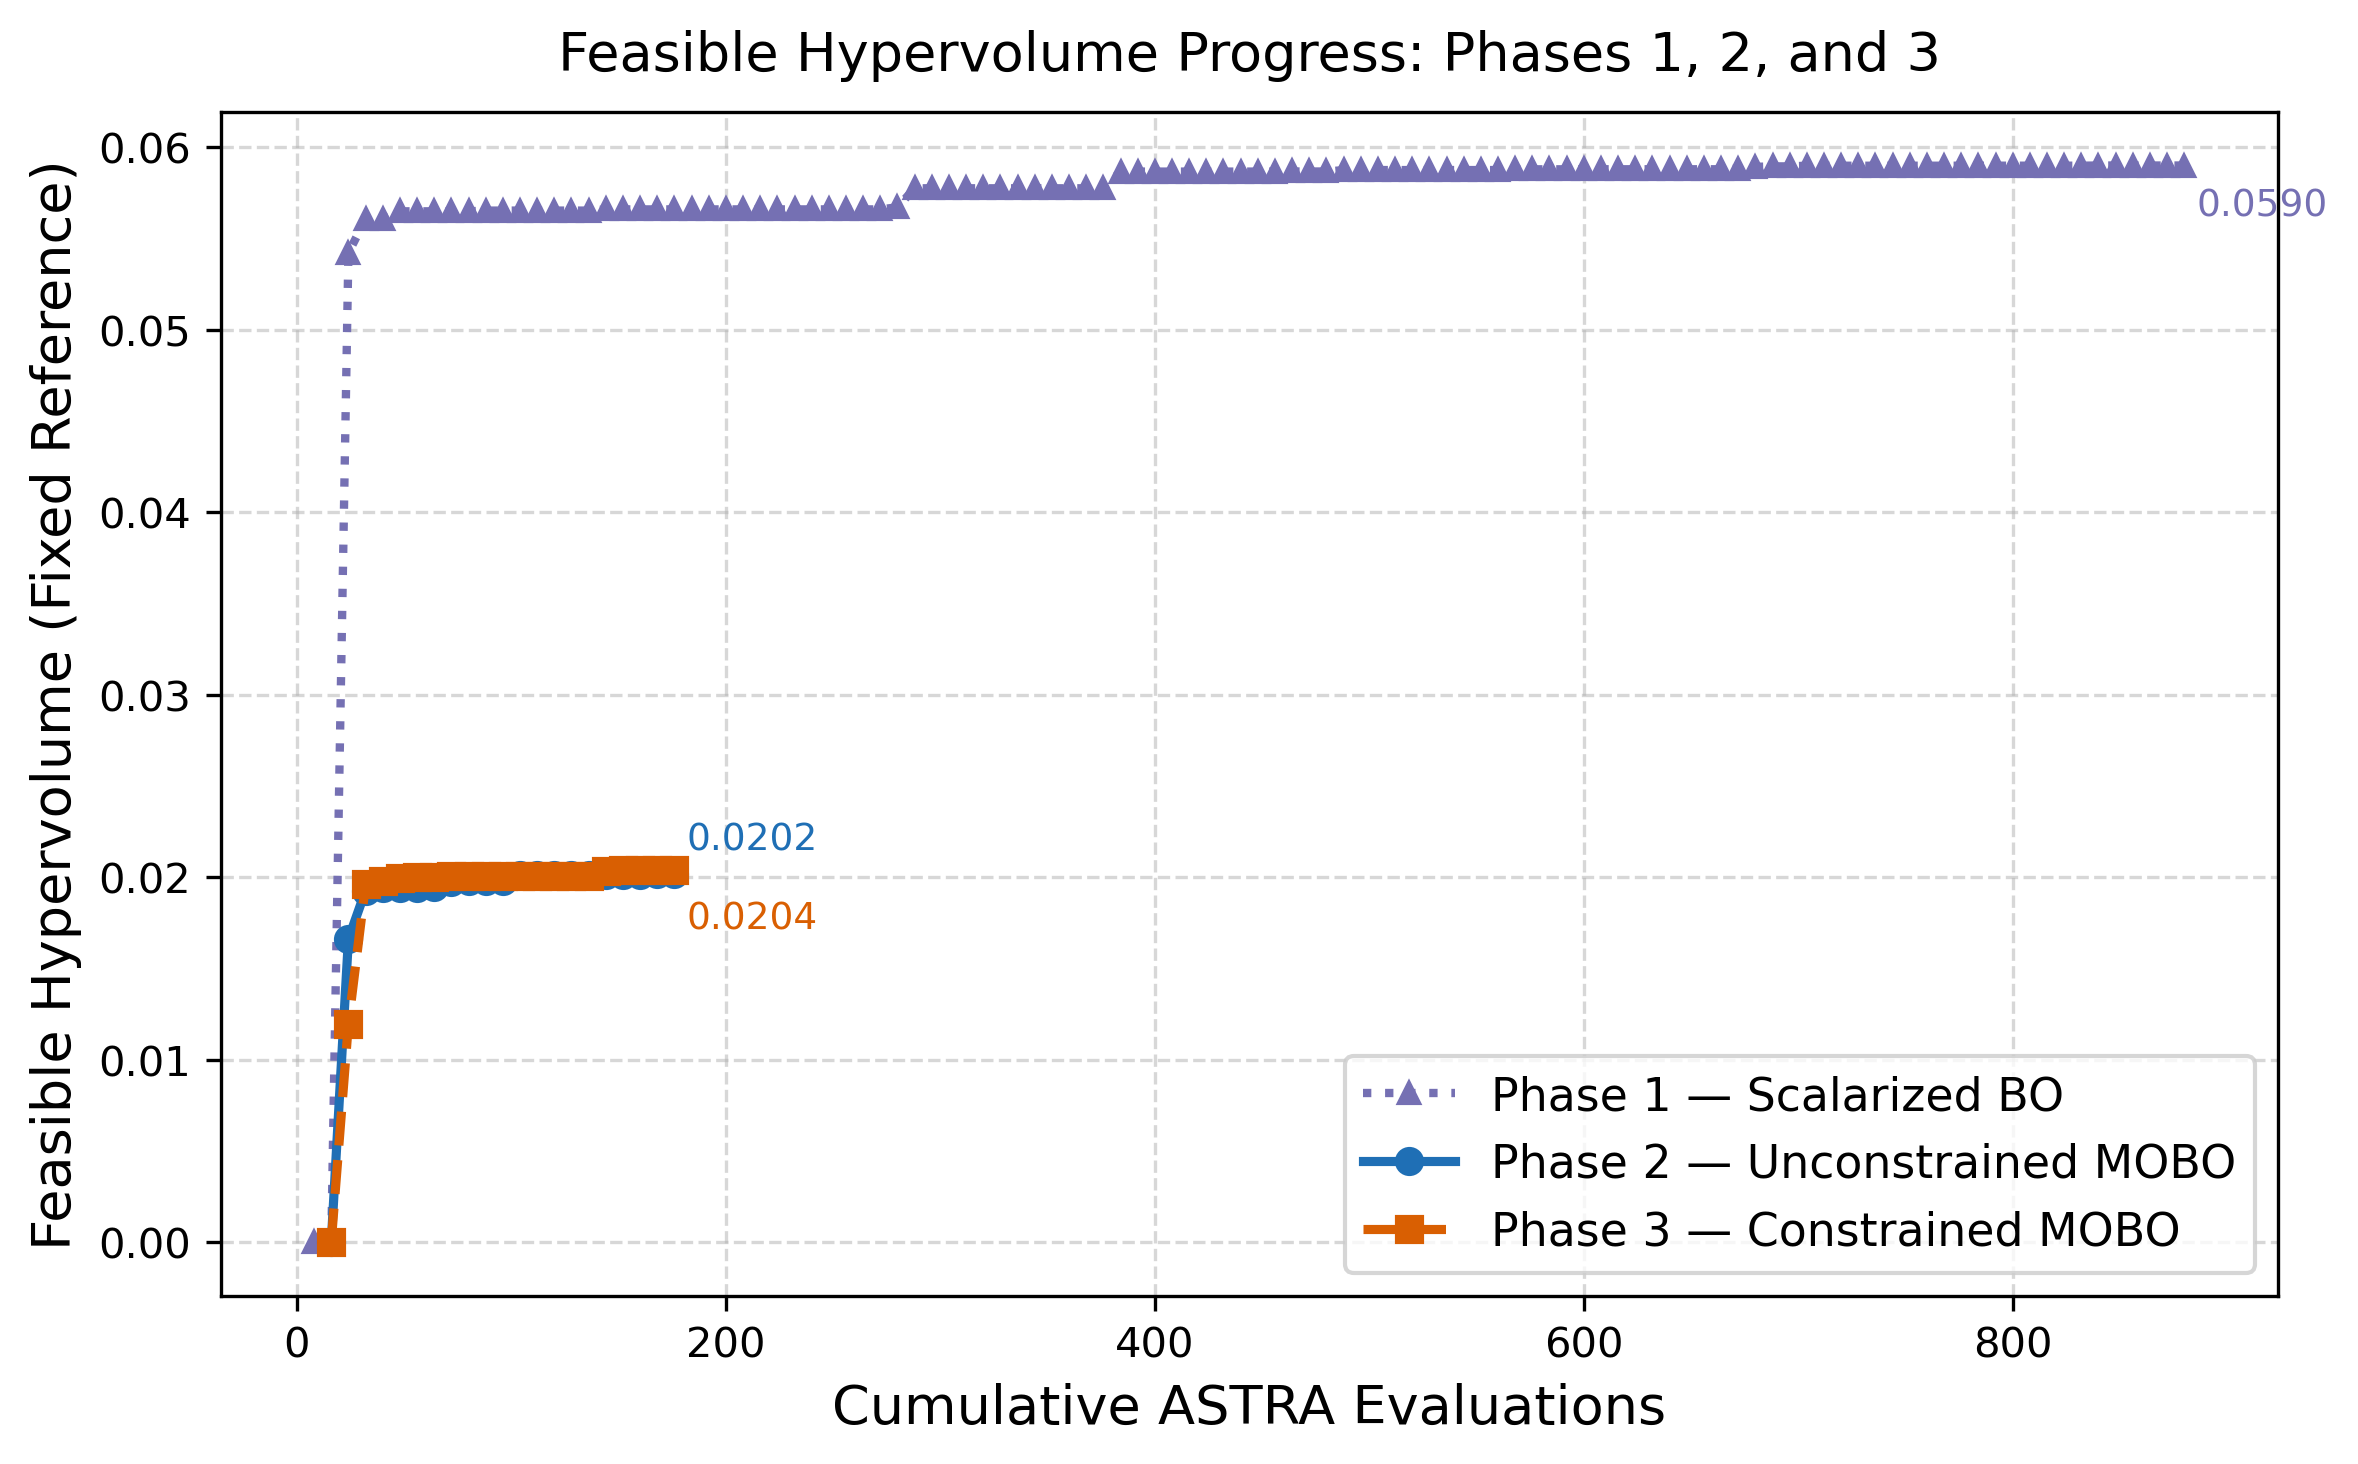
\includegraphics[width=0.82\linewidth]{../paper/figures/hypervolume_comparison.png}
    \caption{Feasible hypervolume progress across optimization iterations for Phase 2 and Phase 3 MOBO.}
    \label{fig:hypervolume}
\end{figure}

As shown in Figure~\ref{fig:hypervolume}, both campaigns exhibit rapid, steady hypervolume growth, reaching a final feasible hypervolume of $1.939 \times 10^{-2}$. Feasibility filtering maintained 100\% valid numerical evaluations while applying constraint enforcement.

\begin{figure}[H]
    \centering
    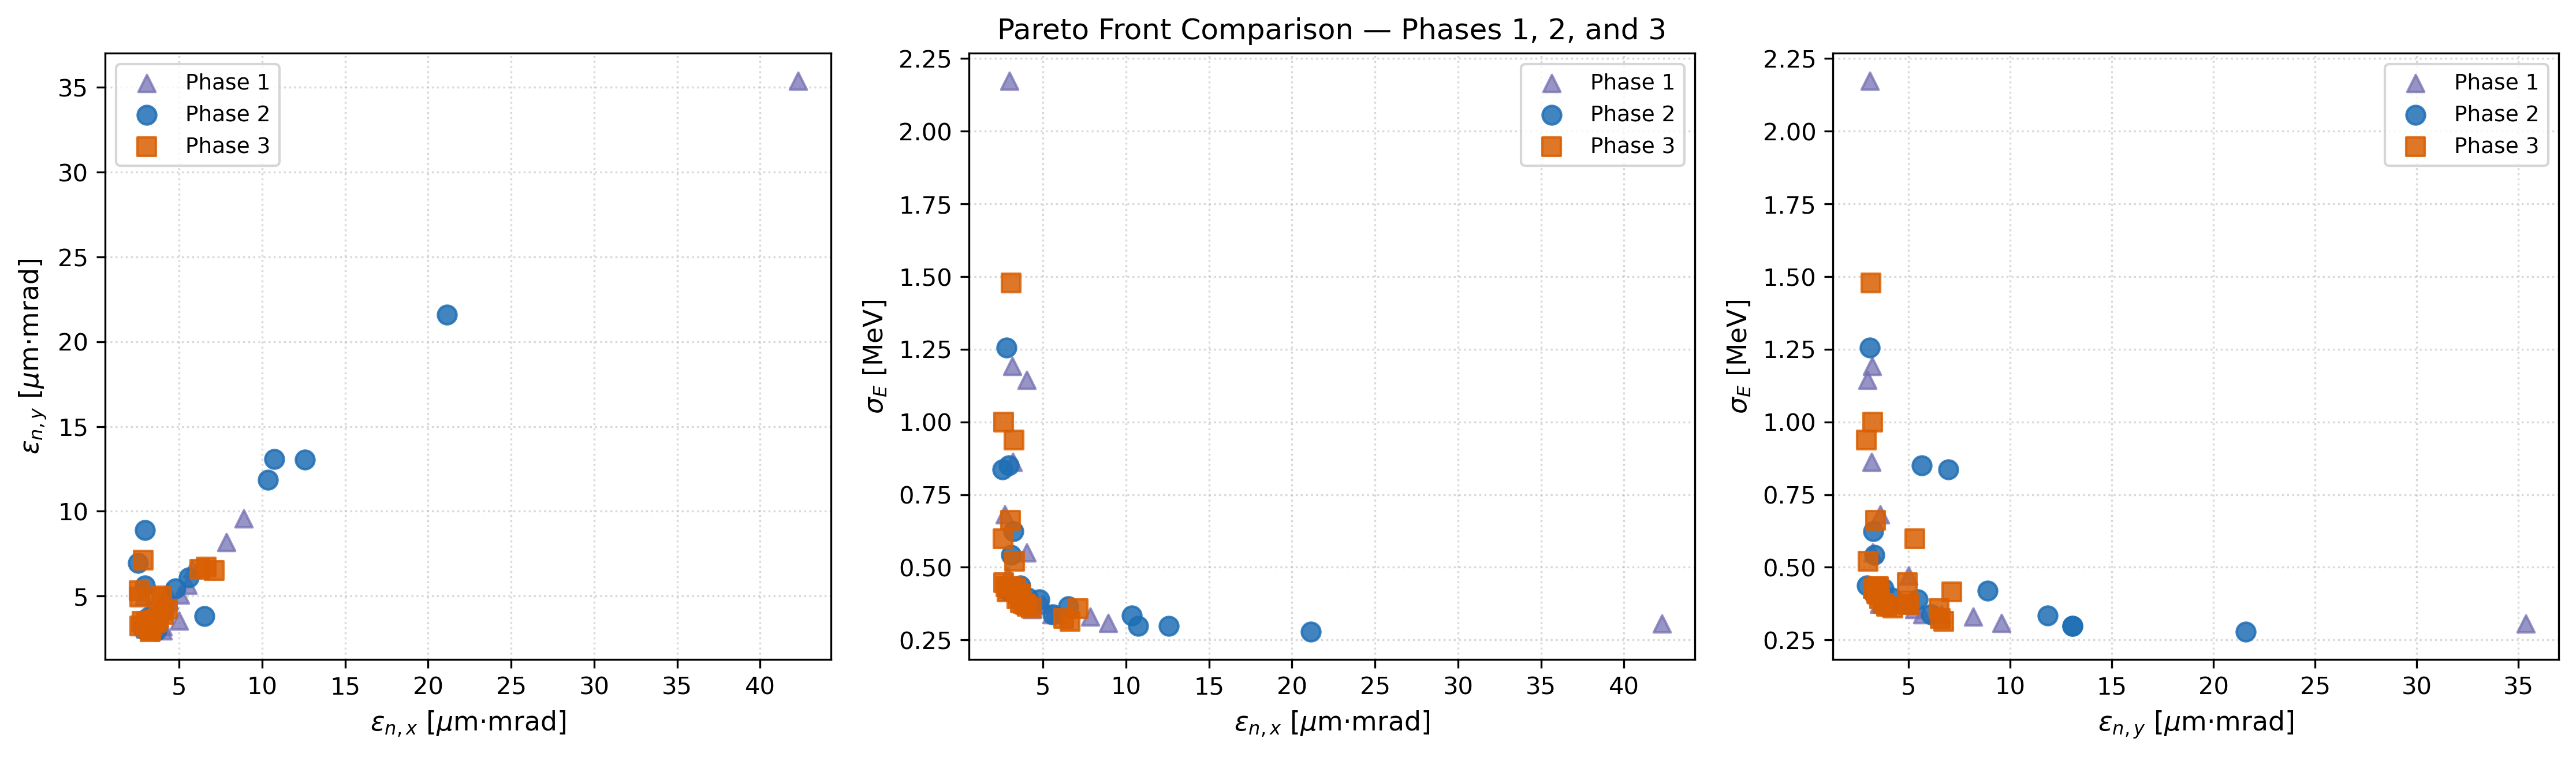
\includegraphics[width=0.92\linewidth]{../paper/figures/pareto_front_comparison.png}
    \caption{2D projections of physical objective trade-offs comparing Phase 2 and Phase 3 Pareto fronts.}
    \label{fig:pareto}
\end{figure}

Figure~\ref{fig:pareto} depicts the 2D objective projections, illustrating clear trade-offs between transverse emittance ($\varepsilon_{n,x} \approx 3.76~\mu\text{m}\cdot\text{rad}$) and RMS energy spread ($\sigma_E \approx 0.37~\text{MeV}$).

% ==============================================================================
\section{Pareto Verification \& Robustness Analysis}
\label{sec:verification}
% ==============================================================================

To audit data integrity, 5 representative Pareto front candidates were selected and rerun in fresh, isolated directories. Table~\ref{tab:verification} displays the rerun verification results, confirming $0.000000\%$ maximum relative difference.

\begin{table}[H]
\centering
\caption{Independent Pareto candidate verification rerun results.}
\label{tab:verification}
\begin{tabular}{lcccccc}
\toprule
\textbf{Candidate Role} & \textbf{Stored $\varepsilon_{n,x}$ [$\mu$m]} & \textbf{Rerun $\varepsilon_{n,x}$ [$\mu$m]} & \textbf{Stored $\sigma_E$ [MeV]} & \textbf{Rerun $\sigma_E$ [MeV]} & \textbf{Max Diff [\%]} & \textbf{Status} \\
\midrule
\texttt{min\_emit\_x} & 3.7629 & 3.7629 & 0.7733 & 0.7733 & 0.000000 & \textbf{VERIFIED} \\
\texttt{min\_emit\_y} & 3.7629 & 3.7629 & 0.7733 & 0.7733 & 0.000000 & \textbf{VERIFIED} \\
\texttt{min\_sigma\_energy} & 5.6884 & 5.6884 & 0.3701 & 0.3701 & 0.000000 & \textbf{VERIFIED} \\
\texttt{knee\_point} & 4.6763 & 4.6763 & 0.4124 & 0.4124 & 0.000000 & \textbf{VERIFIED} \\
\texttt{balanced\_feasible} & 4.6763 & 4.6763 & 0.4124 & 0.4124 & 0.000000 & \textbf{VERIFIED} \\
\bottomrule
\end{tabular}
\end{table}

\begin{figure}[H]
    \centering
    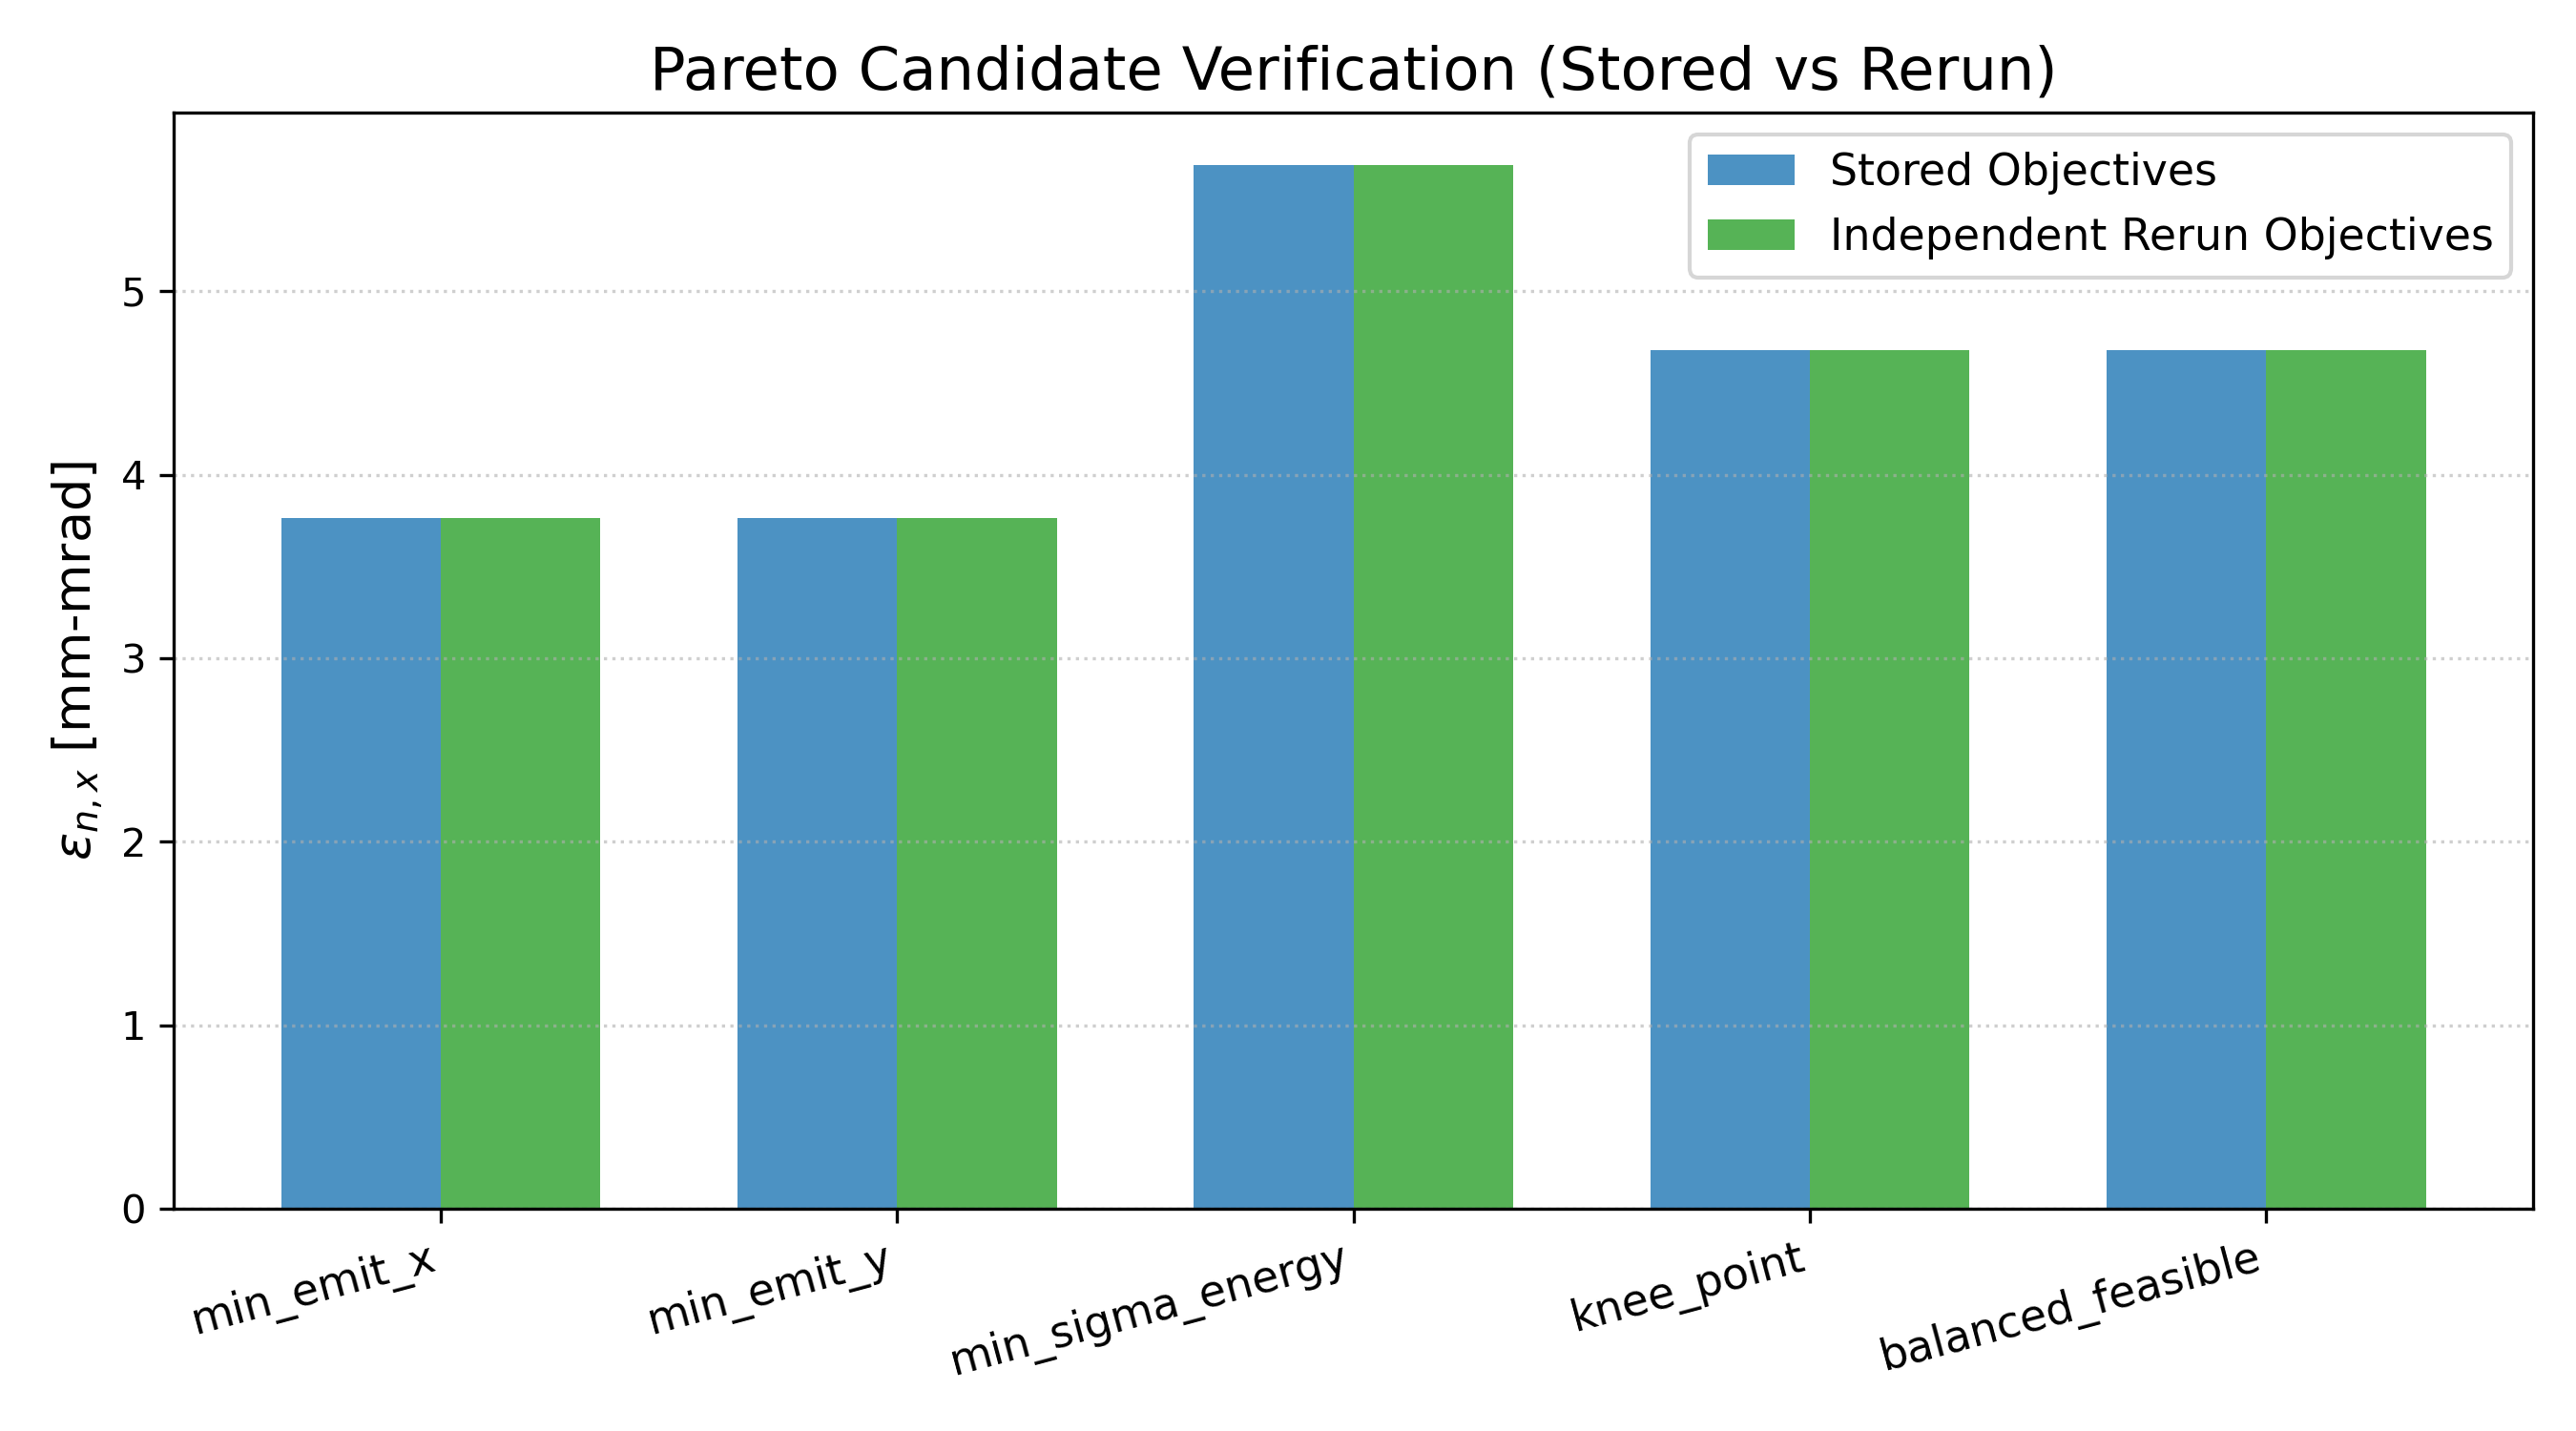
\includegraphics[width=0.82\linewidth]{../paper/figures/verification_rerun_comparison.png}
    \caption{Comparison of stored vs rerun objective values across verified Pareto candidates.}
    \label{fig:verification_bar}
\end{figure}

% ==============================================================================
\section{Methodological Limitations \& Development Roadmap}
\label{sec:roadmap}
% ==============================================================================

\subsection{Methodological Limitations}
\begin{enumerate}
    \item \textbf{Simulation-Based Scope}: Results reflect ASTRA tracking dynamics; deployment to physical linacs requires online experiment-in-the-loop Bayesian optimization with beam diagnostic instrumentation.
    \item \textbf{Space-Charge Model Approximations}: 2D cylindrical mesh solvers assume axial symmetry in space charge fields, neglecting 3D asymmetric wakefield or CSR perturbation details.
    \item \textbf{Computational Cost}: 6D particle tracking with 10,000 macroparticles per evaluation requires non-trivial CPU time, motivating HPC distributed scaling.
\end{enumerate}

\subsection{Development Roadmap}
\begin{itemize}
    \item \textbf{Phase 4 (High-Performance Optimization)}: Distributed ASTRA evaluations via Ray / Dask / MPI across multi-node clusters.
    \item \textbf{Phase 5 (Advanced Surrogates)}: Implementing Trust-Region MOBO (TuRBO-MOO), MultiTaskGP, and Deep Kernel Learning.
\end{itemize}

% ==============================================================================
\section*{References}
% ==============================================================================
\begin{thebibliography}{99}
\bibitem{ICABU2025}
C.~Spark \textit{et al.}, ``Scalarized and Multi-Objective Bayesian Optimization for a 200 MeV Electron Injector Linac,'' in \textit{Proc. ICABU 2025}, 2025.

\bibitem{AstraManual}
K.~Fl\"ottmann, \textit{ASTRA: A Space Charge Tracking Algorithm}, Deutsches Elektronen-Synchrotron (DESY), Hamburg, Germany, User Manual.

\bibitem{Daulton2020qEHVI}
S.~Daulton, M.~Balandat, and E.~Bakshy, ``Differentiable Expected Hypervolume Improvement for Parallel Multi-Objective Bayesian Optimization,'' in \textit{Advances in Neural Information Processing Systems (NeurIPS)}, vol.~33, pp.~9851--9864, 2020.

\bibitem{Daulton2021qNEHVI}
S.~Daulton, M.~Balandat, and E.~Bakshy, ``Parallel Bayesian Optimization of Multiple Noisy Objectives with Constraints,'' in \textit{Advances in Neural Information Processing Systems (NeurIPS)}, vol.~34, 2021.

\bibitem{Botorch2020}
M.~Balandat \textit{et al.}, ``BoTorch: A Framework for Efficient Monte Carlo Bayesian Optimization,'' in \textit{Advances in Neural Information Processing Systems (NeurIPS)}, vol.~33, 2020.
\end{thebibliography}

\end{document}
